\section{Evaluation}
\label{ch:por:sect:eval}

Concerning the evaluation of \coordtool, we focus on two main
aspects. First, we want to understand if the restriction inferring
methodology presented in Section~\ref{ch:por:sect:infer} is effective when being applied to
analyze real world applications, i.e., finding a minimal set of restrictions. 
Second, we need to explore the impacts on user observed latency and system throughput
introduced by the following factors: 

\begin{itemize}
\item adopting PoR-consistent replication
\item using different protocols
\item adding more restrictions
\end{itemize}


\subsection{Case studies}
\label{ch:por:sect:casestudies}
\begin{table}[t!]
\centering
\scriptsize
\begin{tabular}{|l|l|l|}
\hline
App & RedBlue consistency & PoR consistency\\
\hline
\hline
RUBiS & $r(registerUser, registerUser)$ & $r(registerUser, registerUser)$ \\ 
      & $r(storeBuyNow, storeBuyNow)$ & $r(storeBuyNow, storeBuyNow)$\\
      & $r(placeBid, placeBid)$ & $r(placeBid, closeAuction)$\\
      & $r(closeAuction, closeAuction)$ & \\
      & $r(placeBid, closeAuction)$ & \\
      & $r(registerUser, storeBuyNow)$ &\\
      & $r(registerUser, placeBid)$ & \\
      & $r(registerUser, closeAuction)$ &\\
      & $r(storeBuyNow, placeBid)$ & \\
      & $r(storeBuyNow, closeAuction)$ & \\
\hline
\end{tabular}
\caption{Restrictions}
\label{tab:restrict}
\end{table}

We apply the analysis (Algorithm~\ref{alg:mrdiscover}) to a completed version of RUBiS, which
implements a {\tt closeAuction} operation for declaring auction winners, to
identify a set of restrictions comprising a minimal amount of coordination without
sacrificing either state convergence or invariant preservation. This subsection
reports our experience on conducting such analysis and the final static result we
obtained.

\noindent\paragraph{State convergence:} As we deploy RUBiS alongside \tool,
all shadow operations generated at runtime commute w.r.t each other and
there is no need to restrict any pair of shadow operations. The final output of
the state convergence restriction discovery method (Algorithm~\ref{alg:scdiscover}) is an empty restriction set.

\noindent\paragraph{Invariant preservation:} By analyzing the source code, we determined
four invariants of the completed version of RUBiS, namely, (a) identifiers 
assigned by the system are unique; (b) nicknames chosen by
users are unique; (c) item stock must be non-negative; and (d) the auction 
winner must be associated with the highest bid across all accepted bids. We continued by
performing the {\tt I-conflict set} analysis (Algorithm~\ref{alg:iconflictassess}) against all RUBiS shadow operations. With regard
to the first invariant, since we take advantage of the coordination-free unique identifier generation method
offered by \tool, no {\tt I-conflict sets} were found for violating it. In contrast, 
for the remaining three invariants, we identified
the following {\tt I-conflict} sets: 

\begin{itemize}
 \item$\{registerUser', registerUser'\}$. The (b) invariant would
be violated if the two operations proposed the same $nickname$ and were submitted to different sites simultaneously;
 \item $\{storeBuyNow', storeBuyNow'\}$. The (c) invariant would be violated if both operations simultaneously
deducted a positive number from $stock$ while $stock$ was not enough; 
 \item $\{placeBid', closeAuction'\}$. The (d) invariant would be violated if both operations were submitted at the same
time to different sites plus $placeBid'$ carried a higher bid than all accepted bids.
\end{itemize} 
Each of the three above {\tt I-conflict sets} covers a class
of violating executions of the respective invariant. To eliminate these
violations, according to Algorithm~\ref{alg:isdiscover}, we added the following restrictions, namely,
$r(registerUser', registerUser')$, $r(storeBuyNow', storeBuyNow')$ and $r(placeBid', closeAuction')$, 
which are summarized in Table~\ref{tab:restrict}. This set is a minimal restriction
set since it is sufficient to ensure the two important properties while none of these restrictions
can be removed. However, compared to the PoR consistency solution, replicating RUBiS
via RedBlue consistency would require more restrictions, since the definition states that
all non-invariant safe shadow operations must be red (strongly consistent), i.e., the four shadow operations presented
in the above list must be restricted in a pair-wise fashion, as shown in Table~\ref{tab:restrict}. 
\if 0
We have previously introduced an auction service
as a motivating example for the limitations of hybrid consistency models such as
\RBCN. We \changebars{are able to compose an invariant-violating
execution with three concurrent operations touching a shared auction, 
namely, a {\tt close\_auction} operation and
two {\tt place\_bid} operations whose associated bids are higher than
all accepted bids.}{remind the reader that such a service supports two operations, in 
particular a {\tt place\_bid} operation to submit a new bid for an
auction, which is accepted provided that the target auction is not closed; and a {\tt close\_auction}
operation which closes the auction while at the same time declares a winner. 
An application-specific invariant is that the declared winner must be the user
that issued the highest accepted bid (while the auction was not closed).}
\changebars{According to the definition in Section~\ref{sect:intro},
this execution is not minimal since the composition of a {\tt place\_bid}
and {\tt close\_auction} operation is already sufficient to trigger the violation. Thus,
we refine the execution by removing one of the {\tt place\_bid} operations from it.}{} 
As a way to \changebars{preserve}{enforce} 
the \changebars{}{application-specific }invariant of this service under \PRCN\ 
a restriction \changebars{must}{can} be created between \changebars{any pair of a}{operations of type} {\tt place\_bid} and 
\changebars{a}{operations of the type} {\tt close\_auction}\changebars{ operation,
i.e., $r({\tt place\_bid}, {\tt close\_auction})$}{}. 
The advantage of this approach is that \changebars{}{ the instances of}{\tt place\_bid} \changebars{operations}{}
have no restrictions among themselves, which implies that no coordination mechanism is required when executing \changebars{them
concurrently}{several 
instances of this type of operation}. \changebars{Given the fact that these
operations}{ which, incidentally,} are the most common in
such a service\changebars{, performance will be dramatically improved}{}.
\fi
\if 0
\paragraph*{Banking Service} Another interesting example is an
online banking service, that supports operations such as {\tt deposit} and 
{\tt withdraw} which respectively, allows a user to add or remove a given amount to or from
the current bank account balance, while a third operation\changebars{}{ type denominated}
{\tt accrueinterest}, updates the balance value of an account by taking into
consideration its current balance and a given interest rate. \changebars{We further assume}{In this service
one can imagine that there is } an application-specific invariant which states
that account balance values must be non-negative.

In this particular example, to ensure state convergence, \changebars{}{operations
of type}{\tt accrueinterest} operations must be executed with coordination in relation 
to \changebars{}{operations of type}{\tt deposit} or {\tt withdraw} operations\changebars{, i.e.,
creating two restrictions $r({\tt accrueinterest}, {\tt deposit})$
and $r({\tt accrueinterest}, {\tt withdraw})$, as multiplication does not
commute with addition or subtraction.}{ In \PRCN\ this is modeled
by creating two restrictions respectively, between  {\tt accrueinterest} and 
{\tt deposit} and between {\tt accrueinterest} and {\tt withdraw}.}
However to ensure the application-specific invariant, special care has to
given to \changebars{}{operation of the type }{\tt withdraw}\changebars{ operations, as
two concurrent {\tt withdraw} operations may drive the balance value to negative}{}. 
\changebars{As a result}{In fact}, \changebars{}{all instances of }these
operations have to be coordinated among themselves. To capture this 
fact one has to add an additional restriction \changebars{}{to order operations of type
{\tt withdraw}, i.e.,}$r({\tt withdraw}, {\tt withdraw})$. \changebars{}{This approach allows 
operations of type {\tt deposit}
to be executed without any form of coordination
among themselves.}
\fi


\begin{table}[t]
\centering
\scriptsize
 \begin{tabular}{c|l|l|l|}
 & US-East & US-West & EU-FRA \\
\hline
\multirow{2}{*}{US-East} &  $0.299\pm0.042$  ms  & $71.200\pm0.021$ ms    & $88.742\pm1.856$ ms  \\
   &  $1052.0\pm0.0$ Mbps& $47.4\pm1.6$ Mbps & $29.6\pm5.6$ Mbps \\
\hline
\multirow{2}{*}{US-West} &    $66.365\pm0.006$ ms    & $0.238\pm0.003$ ms   & $162.156\pm0.179$ ms \\
   &   $47.4\pm1.6$ Mbps      & $1050.7\pm4.1$ Mbps & $17.4\pm1.7$ Mbps  \\
\hline
\multirow{2}{*}{EU-FRA} &   $88.168\pm0.035$ ms     &   $162.163\pm0.157$ ms   & $0.226\pm0.003$ ms  \\
   &    $36.2\pm0.1$ Mbps     &     $20.1\pm0.1$ Mbps     & $1052.0\pm0.0$ Mbps \\
\hline
\end{tabular}
\caption{Average round trip latency and bandwidth between Amazon datacenters (obtained in Dec 2015).}
\label{tab:por:roundtriplatency}
\end{table}


\subsection{Experimental setup}
\paragraph{Deployment parameters:}
We run experiments on Amazon EC2~\cite{AmazonEC2} using {\tt m4.2xlarge} virtual machine instances
located in three sites: US Virginia (US-East), US California (US-West) and EU Frankfurt (EU-FRA), which
are the latest generation of General Purpose Instances. Table~\ref{tab:por:roundtriplatency} shows the 
average round trip latency and observed bandwidth between every pair of sites. Each VM has 8 virtual cores 
and 32GB of RAM. VMs run Debian 8 (Jessie) 64 bit, MySQL 5.5.18, Tomcat 6.0.35, and OpenJDK 8 software. 

\paragraph{Configuration and workloads:}
Unless stated otherwise, in all experiments, we deploy the BFTSmart library under the crash-fault-tolerance
model (CFT) with 3 replicas across three sites, and assign the replica at EU-FRA to act as the leader of the Paxos protocol. 
We replicate RUBiS under PoR consistency across three sites using \coordtool, \tool, and \Gemini,
while running an unreplicated strongly consistent RUBiS in the EU-FRA site as a baseline. We refer
the first experiment to ``\coordtool-3-datacenter'', and the second experiment to ``Unreplicated''.
For all experiments, emulated clients are equally distributed across three sites and connect
to their closest data center by physical proximity. 

We choose to run the bidding mix workload of RUBiS, where 15\% of user interactions 
are updates. To make the client emulator issue the newly introduced {\tt closeAuction}
requests, we have to slightly change the transition table equipped with the original RUBiS code
by assigning a positive probability value for this request. The new transition table can be found here~\cite{OlisipoTranstionTable}.
For all experiments we vary the workload by increasing the number of concurrent client threads in every client emulator.
We also disable the {\tt thinking time} option for issuing requests so that
there is no waiting time between two contiguous requests from the same client thread.
With regard to the data set, we populate it via the following parameters: the RUBiS database contains 33,000 items for sale, 1 million
users, and 500,000 old items.

\subsection{Experimental results}
In this part, we analyze the results obtained from running experiments stated above concerning
the following aspects.
\subsubsection{Overall performance}
\begin{figure}[t!]
  \centering
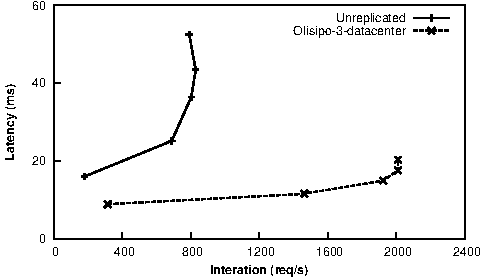
\includegraphics[width=0.85\columnwidth]{figures/eval/throughput_unreplicated_vs_por.pdf}
  \caption{Throughput versus latency curves for the RUBiS bidding mix.}
 \label{fig:por:thptunreplicatevspor}
\end{figure}

We start by looking into the overall performance comparison between a 3 site \coordtool\ deployment of
RUBiS, which offers fine-grained tradeoffs between consistency and performance, and a single site original code deployment,
which provides strong consistency. Figure~\ref{fig:por:thptunreplicatevspor} shows the overall average latency and throughput curves of the
two experiments. Olisipo significantly outperforms the unreplicated RUBiS deployment in two dimensions,
namely, \coordtool\ reduces average latency (44.3\% lower for the first data point from left to right) and improves peak throughput (142.8\% higher).
The performance gains come from the fact that \coordtool\ is able to execute most of (non-conflicting) requests 
in a coordination-free manner and to call efficient coordination policy when needed for processing conflicting requests.

\subsubsection{User perceived latency}
The major concern of designing Olisipo is to reduce the user perceived latency. In order
to understand the effectiveness of \coordtool\ on this front, we break down the overall latency shown in Figure~\ref{fig:por:thptunreplicatevspor}
into the following categories.
\begin{figure}[t!]
  \centering
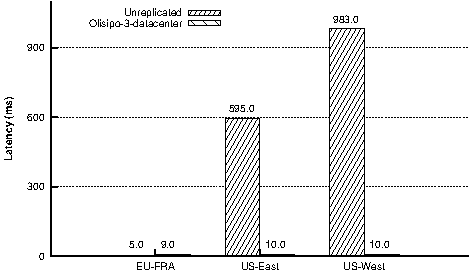
\includegraphics[width=0.85\columnwidth]{figures/eval/avg_latency_unreplicated_vs_por.pdf}
  \caption{Overall average latency bar graph for users located in three sites.}
 \label{fig:por:avglatenunreplicatevspor}
\end{figure}
\paragraph{{\em Per data center basis:}} First, we analyze the average latency
for users at each data center, respectively. As shown in Figure~\ref{fig:por:avglatenunreplicatevspor},
all users except those in EU-FRA observe notably lower latency in the Olisipo experiment, compared
to the users from the same locations in the unreplicated experiment. This improvement is because in \coordtool, most of
requests are handled locally, while in the unreplicated RUBiS, requests from users at
two US data centers have to be redirected to EU-FRA, which incurs expensive inter-datacenter communication. Unlike users at these two data centers, we also
observed that users at EU-FRA in the Olisipo experiment experience a slightly higher latency than users
from the same region accessing an unreplicated RUBiS. This can be explained by the additional work required
for incorporating remote shadow operations into the local causal serialization and placing coordination if needed for
serializing conflicting requests. Although the Olisipo user observed latency at EU-FRA is almost twice as
big as the latency of the unreplicated experiment, the absolute number (9 ms) is reasonably low.

\begin{figure}[t!]
  \centering
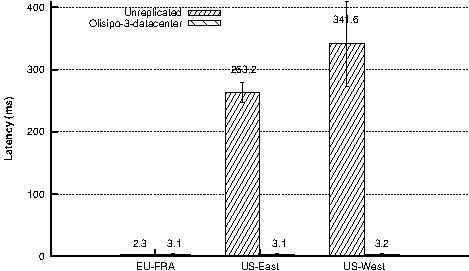
\includegraphics[width=0.85\columnwidth]{figures/eval/avg_latency_storecomment_unreplicated_vs_por.pdf}
  \caption{Average latency bar graph of a RUBiS request {\tt storeComment} for users located at three sites. In
  the context of \PRCN, this request is non-conflicting and hence does not require coordination.}
 \label{fig:por:avglatennfunreplicatevspor}
\end{figure}

\paragraph{{\em Latency of non-conflicting requests: }}Second, we try to understand the impact
on latency observed by non-conflicting requests. Among all non-conflicting requests in RUBiS,
we chose one representative request called {\tt storeComment} as the illustrating example, which places
a comment on a user profile. As depicted in Figure~\ref{fig:por:avglatennfunreplicatevspor}, the conclusion we can draw from this graph
is consistent with the one regarding Figure~\ref{fig:por:avglatenunreplicatevspor}. However, the major
difference between these two figures is that users from EU-FRA in both experiments have almost identical
latency. This is because the request {\tt storeComment} requires no coordination and the cost of 
generating and applying the corresponding shadow operation is modest.

\begin{figure}[t!]
  \centering
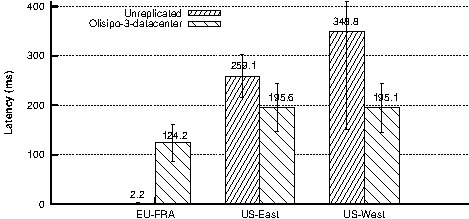
\includegraphics[width=0.85\columnwidth]{figures/eval/avg_latency_sym_storebuynow_unreplicated_vs_por.pdf}
  \caption{Average latency bar graph of a RUBiS request {\tt storeBuyNow} for 
  users located at three sites. In
  the context of \PRCN, {\tt storeBuyNow} conflicts w.r.t itself and is regulated by the {\tt Sym} protocol when being replicated.}
 \label{fig:por:avglatensymunreplicatevspor}
\end{figure}

\paragraph{{\em Latency of conflicting requests: }} Third, we shift our attention from non-conflicting requests
to conflicting ones. As introduced before, equipping with different coordination 
protocols would lead to different performance loss. We start by analyzing the latency of 
requests handled by the {\tt Sym} protocol. The illustrative example we selected 
is {\tt storeBuyNow}, which is conflicting with respect to itself. As shown in 
Figure~\ref{fig:por:avglatensymunreplicatevspor}, in the Olisipo experiments, all users 
from all three sites observe extraordinarily higher latency, which is between 100 ms to 200 ms, compared
to non-conflicting requests (shown in Figure~\ref{fig:por:avglatennfunreplicatevspor}), 
whose latency is under 10 ms. This is because most of the lifecycle of these
requests was spent asking a centralized counter service for granting permissions, which
consists of 3 replicas spanning three sites and executing a Paxos-like consensus protocol. 
Additionally, user observed latency at EU-FRA is lower than
the remaining two sites, since the leader of the consensus protocol is co-located
with EU-FRA users. 

\begin{figure}[t!]
  \centering
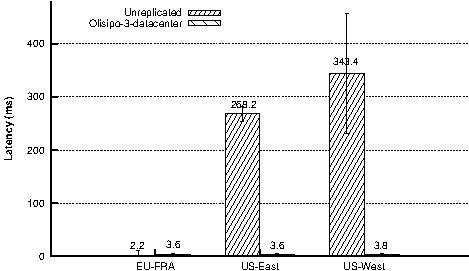
\includegraphics[width=0.85\columnwidth]{figures/eval/avg_latency_asym_placebid_unreplicated_vs_por.pdf}
  \caption{Average latency bar graph of a conflicting request {\tt placeBid} for
  users locating in three sites, which is conflicting with {\tt closeAuction'}. This request
  is regulated by the {\tt Asym} protocol but is not a barrier.}
 \label{fig:por:avglatenasymnbunreplicatevspor}
\end{figure}

We continue by understanding how the average latency of {\tt Asym} requests looks like. 
Unlike the {\tt Sym} protocol, any pair of operations confined in a restriction 
will be treated differently by the {\tt Asym} protocol, namely one acts
as a distributed barrier and the other proceeds if no active barriers are running. 
In the case study section (Section~\ref{ch:por:sect:casestudies}), we assign 
the {\tt Asym} protocol to regulate the $r(placeBid', closeAuction')$ restriction while 
the less frequent shadow operation $closeAuction'$ works as a barrier. As shown in 
Figure~\ref{fig:por:avglatenasymnbunreplicatevspor}, the average latency 
measured for the $placeBid$ request, which produces $placeBid'$, looks very similar
with the results obtained for non-conflicting requests shown in Figure~\ref{fig:por:avglatennfunreplicatevspor}.
The is because the ratio of $closeAuction$ to
$placeBid$ is very low (2.7\%) and most of time the $placeBid$ request 
commits immediately without waiting for joining or leaving barriers. 
\begin{figure}[t!]
  \centering
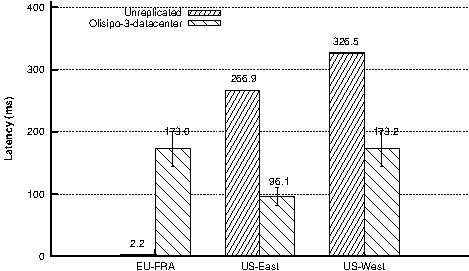
\includegraphics[width=0.85\columnwidth]{figures/eval/avg_latency_asym_closeauction_unreplicated_vs_por.pdf}
  \caption{Average latency bar graph of a conflicting request {\tt closeAuction},
  which is conflicting with {\tt placeBid}. This request is handled by the {\tt Asym}
  protocol and acts as the barrier.}
 \label{fig:por:avglatenasymbunreplicatevspor}
\end{figure}


Next, we consider the barrier request $closeAuction$ handled by 
the {\tt Asym} protocol. As expected, compared to $placeBid$, the average 
latency of $closeAuction$ is remarkably higher due to
the coordination across sites, through which this request forces all sites not to
process incoming $placeBid$ requests and collecting results of all relevant
completed $placeBid$ requests. As shown in 
Figure~\ref{fig:por:avglatenasymbunreplicatevspor}, users issuing
$closeAuction$ observed a latency slightly higher than the maximal RTT between 
their primary data center and the remaining data centers. For example, 
as shown in Table~\ref{tab:por:roundtriplatency}, the maximal RTT for US-East users
is 88.7 ms, while the latency of $closeAuction$ observed by 
the same group of users is 96.1 ms.

\begin{figure}[t!]
\centering

\subfloat[\textsf{Peak throughput}]{
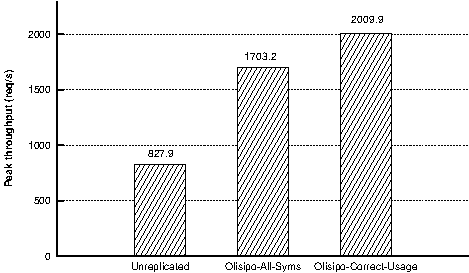
\includegraphics[width=0.85\columnwidth]{figures/eval/peakthroughput_allsym_vs_right.pdf}
\label{fig:por:pkthptallsymvsright}
}
\\
\subfloat[\textsf{Overall average latency}]{
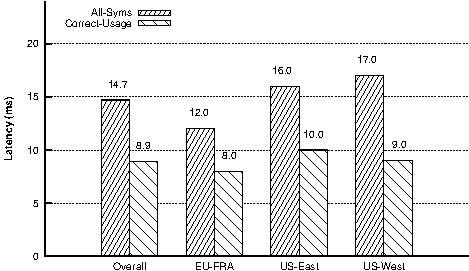
\includegraphics[width=0.85\columnwidth]{figures/eval/avg_latency_allsym_vs_right.pdf}
\label{fig:por:avglatenallsymvsright}
}
\caption{Peak throughput and overall average latency bar graphs of systems using different protocols.}
\label{fig:por:allsymvsright}
\end{figure}

\subsubsection{Impact of different protocols}
As motivated in the design of \coordtool, the purpose of offering different coordination protocols is
to additionally improve runtime performance by taking into account the workload metrics. To validate this, we deploy
another baseline experiment denoted by {\tt \coordtool-All-Syms}, in which the restriction $r(placeBid', closeAuction')$
is also regulated by the {\tt Sym} protocol. In addition, we denote the experiment where
the protocol assignment is done properly as {\tt \coordtool-Correct-Usage}, i.e., $r(placeBid', closeAuction')$ is handled
by the {\tt Asym} protocol. Figure~\ref{fig:por:allsymvsright} summarize the comparison of peak throughput and average latency among
three experiments, namely, {\tt Unreplicated}, {\tt \coordtool-All-Syms} and {\tt \coordtool-Correct-Usage}. As expected, the performance
achieved by {\tt \coordtool-All-Syms} is between {\tt Unreplicated} and {\tt \coordtool-Correct-Usage}. On the one hand,
it indeed improves peak throughput of the unreplicated RUBiS by 105.7\%, because of the coordination-free execution of non-conflicting
requests. However, on the other hand, compared to {\tt \coordtool-Correct-Usage}, the performance of {\tt \coordtool-All-Syms} degrades in
two dimensions, namely, 15.3\% decrease in peak throughput
and 65.2\%, 50.0\%, 60.0\%, 88.9\% increase in request latency for all, EU-FRA, US-East, US-West users, respectively. The reason for
this performance loss is as follows: due to the inappropriate protocol selection, every {\tt placeBid'} shadow operation in {\tt \coordtool-All-Syms} requires a communication
step between its primary site and the centralized counter service for being coordinated, while most of time {\tt placeBid'} shadow operations in 
{\tt \coordtool-Correct-Usage} work as non-conflicting requests provided that {\tt closeAuction} requests sparsely arrive in the system. 


\begin{figure}[t!]
\centering

\subfloat[\textsf{Peak throughput}]{
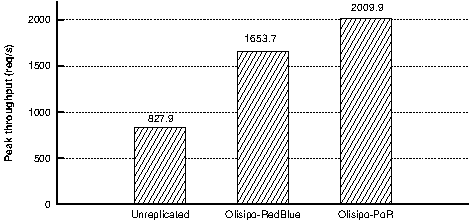
\includegraphics[width=0.85\columnwidth]{figures/eval/peakthroughput_redblue_vs_por.pdf}
\label{fig:por:pkthptredbluevspor}
}
\\
\subfloat[\textsf{Overall average latency}]{
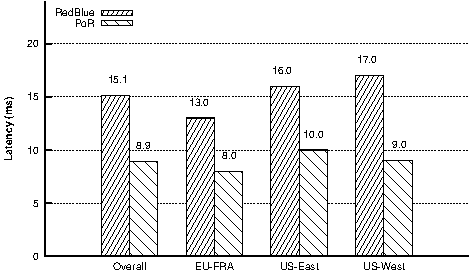
\includegraphics[width=0.85\columnwidth]{figures/eval/avg_latency_redblue_vs_por.pdf}
\label{fig:por:avglatenredbluevspor}
}
\caption{Peak throughput and overall average latency bar graphs of RedBlue consistency and PoR consistency.}
\label{fig:por:redbluevspor}
\end{figure}

\subsubsection{Impact of the number of restrictions}
The last aspect of our evaluation is to explore the impact on latency and throughput introduced by variation in the number
of restrictions. To this end, we deploy a baseline experiment denoted by {\tt RedBlue}, in which
we replicate RUBiS via the PoR consistency framework but with the set of restrictions (shown in Table~\ref{tab:restrict}) we identified for offering
RedBlue consistency. The comparison among the unreplicated RUBiS, RedBlue-consistent RUBiS
and PoR-consistent RUBiS is summarized in Figure~\ref{fig:por:redbluevspor}. As shown in Figure~\ref{fig:por:pkthptredbluevspor}
a 3 site RedBlue replication
improves peak throughput offered by the unreplicated strongly-consistent solution by 99.7\%. However, compared to
PoR, due to unnecessary restrictions enforced by RedBlue consistency, it achieves worse performance, namely, 19.2\% decrease in peak throughput
and 67.8\%, 62.5\%, 60.0\%, 88.9\% increase in request latency for all, EU-FRA, US-East, US-West users, respectively.





